\section{Analysis}
\label{sec:analysis}

\begin{figure}[t]
    \centering
    \vspace{-3mm}
    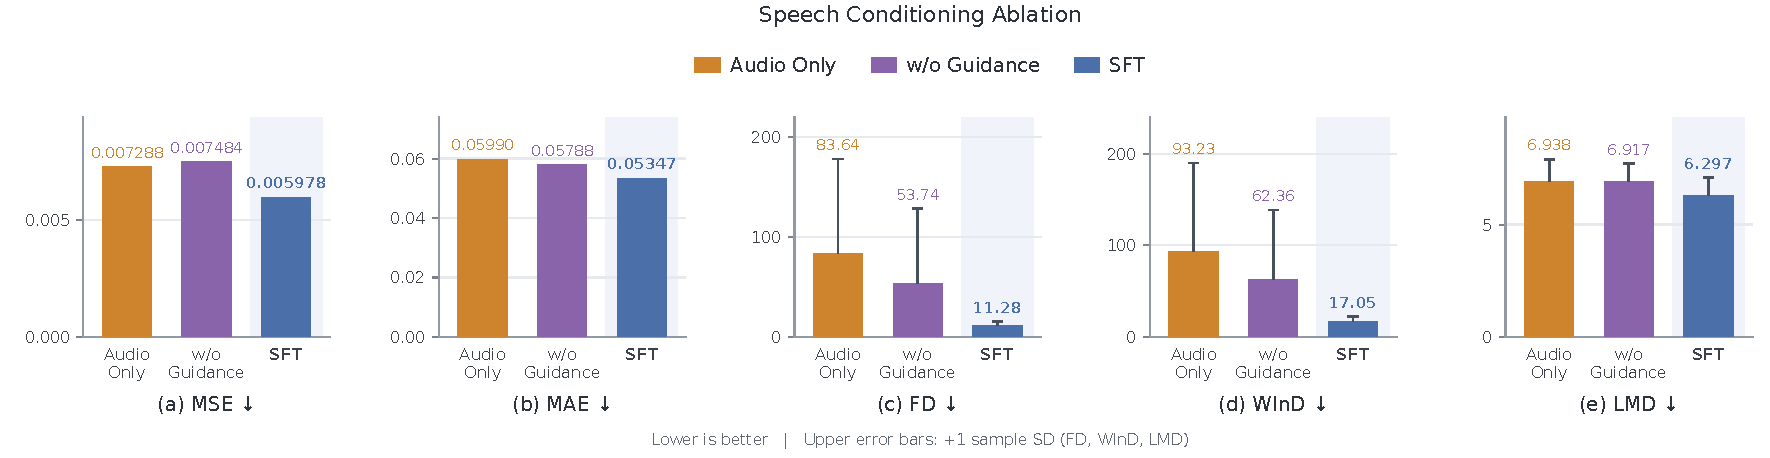
\includegraphics[width=0.82\linewidth]{figures/ablation_conditioning_wide.pdf}\\[0.6mm]
    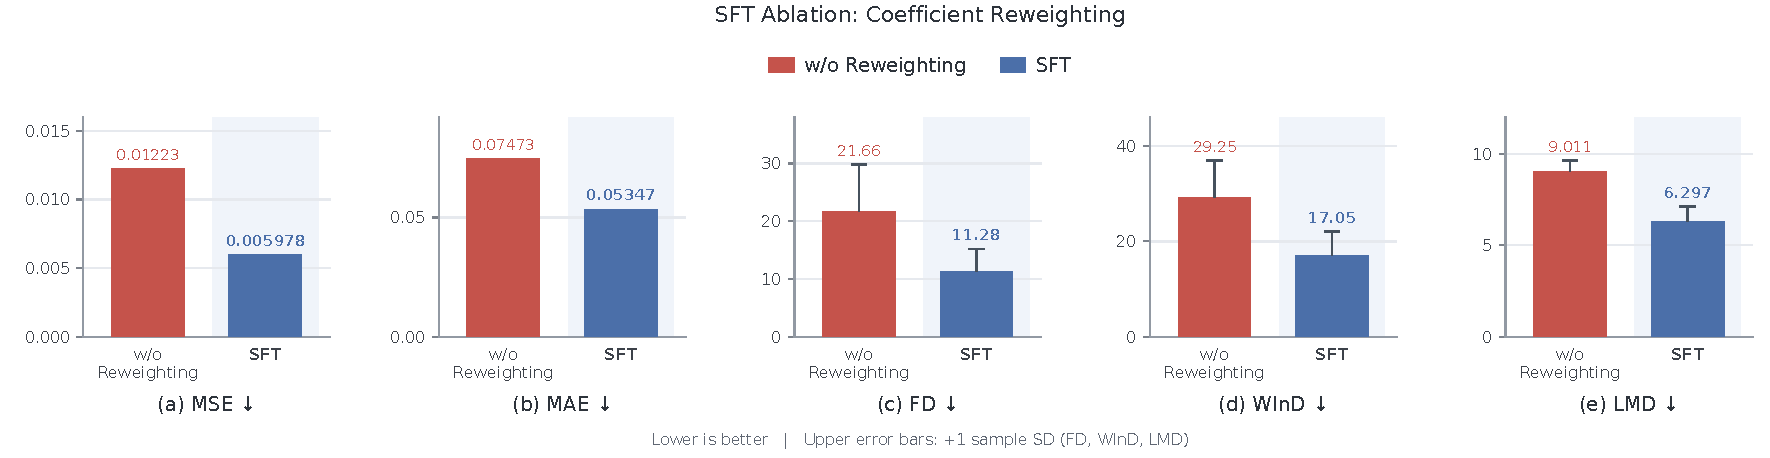
\includegraphics[width=0.82\linewidth]{figures/ablation_reweighting_wide.pdf}
    \vspace{-2mm}
    \caption{The two supervised-stage components act on different failure modes. Removing articulation grounding (top) costs little frame-level error while inflating the distributional metrics and their across-script variance by an order of magnitude, whereas removing the balanced objective (bottom) keeps motion in the right channels yet shrinks its amplitude, which doubles frame-level error and yields the worst rendered landmark distance we measure. Lower is better, and error bars show one sample standard deviation.}
    \label{fig:ablation_sft}
    \vspace{-5mm}
\end{figure}

\subsection{Ablation Study on Articulation Grounding}
\label{sec:ana_conditioning}

To verify that the gain of AudioMouth comes from articulation grounding instead of from the capacity of the multimodal backbone, we ablate the linguistic inputs while holding the backbone, the training data, the objective, and the post-processing identical. The full model receives audio, transcript, phonemes, and the grounding statement. The w/o Guidance variant keeps transcript and phonemes but deletes the statement naming which control each phoneme group drives, and the Audio Only variant deletes all three, which reduces the model to a structured audio-to-coefficient regressor.

As shown in the top row of Figure~\ref{fig:ablation_sft}, the three settings differ by at most a quarter in MSE and about a tenth in MAE, yet by almost an order of magnitude in FD and WInD, where the full model significantly reduces FD by about 79\% relative to w/o Guidance. Notably, the across-script standard deviation grows from a few units for the full model to a value comparable to the mean itself once grounding is removed, a size that cannot describe uniformly degraded motion and instead indicates that the ungrounded variants track speech acceptably on most scripts and then drift badly on some of them. Without a statement connecting phonemes to named controls, the model has no anchor telling it which channels a sound may activate, so when acoustic evidence is ambiguous it settles on a channel combination that is numerically close yet articulatorily wrong. Phonemes alone recover part of that anchor by narrowing the set of sounds produced, which is why w/o Guidance already cuts the FD of Audio Only by more than a third while the two stay comparable at the frame level. The results show that the benefit of linguistic conditioning comes mainly from naming the articulatory action and not from supplying extra input features, demonstrating the advantage of articulation grounding over feature-level linguistic conditioning.

\subsection{Superiority of Distribution-Balanced Supervision}
\label{sec:ana_reweight}

To verify that reweighting coefficient-value tokens addresses the value imbalance identified in Sec.\ref{sec:stage2}, we compare the balanced objective of Eq.(\ref{eq:db}) with a w/o Reweighting variant assigning unit weight to every coefficient-value token, holding conditioning, schema, and post-processing fixed so the comparison isolates the objective.

As shown in the bottom row of Figure~\ref{fig:ablation_sft}, removing the weighting roughly doubles MSE and, more strikingly, raises LMD above every baseline in Table~\ref{tab:main}, including methods whose own coefficient error is nearly twice as large. This combination is only possible for one reason. Under unit weights the loss is dominated by frequent near-zero targets, so the model converges to a solution that is nearly always right about inactivity and too small whenever motion is required. The rendered face therefore moves in the right places and by too little, which a landmark metric on pixels punishes far more than a coefficient metric on numbers. The distributional metrics agree, since FD degrades but stays well below the ungrounded variants of Sec.\ref{sec:ana_conditioning}, so the channel pattern learned from grounding survives while its amplitude does not. The results show that grounding and balanced supervision act on different failure modes, where the former decides which controls move and the latter decides how far, demonstrating the advantage of combining both in a language model that emits quantized motion.

\begin{figure}[t]
    \centering
    \vspace{-3mm}
    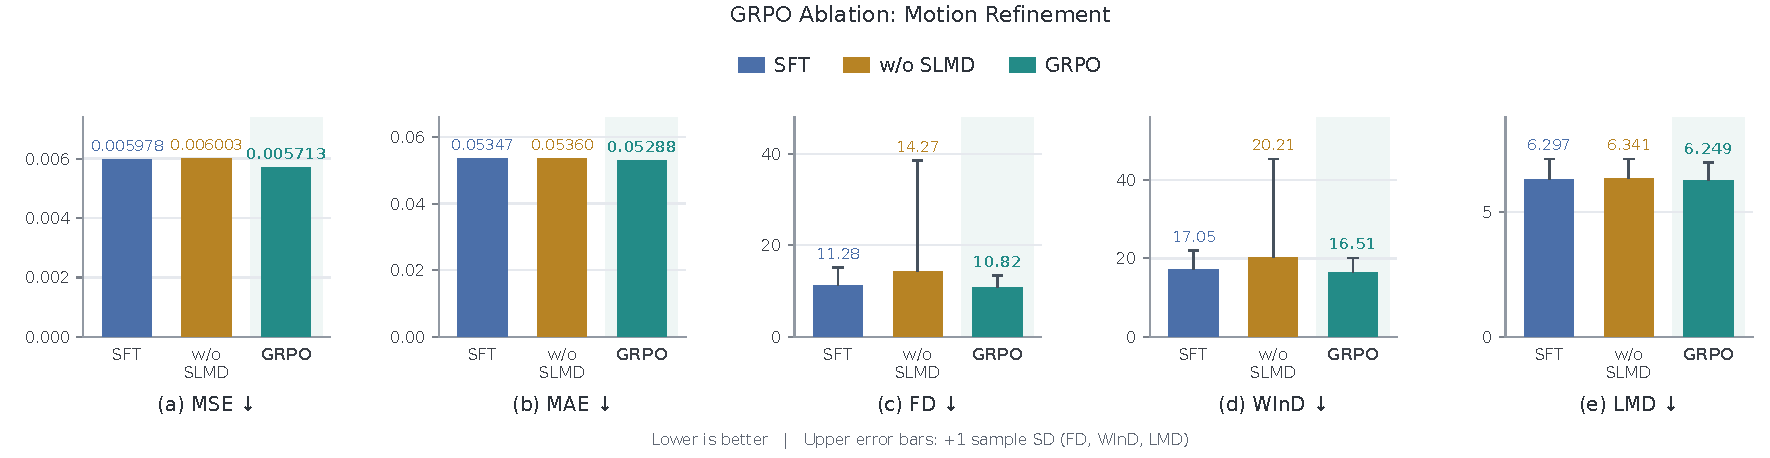
\includegraphics[width=0.82\linewidth]{figures/ablation_motion_wide.pdf}
    \vspace{-2mm}
    \caption{Motion-aware refinement improves consistency more than means. Full refinement gives small gains on every metric and cuts across-script FD deviation by a third, while dropping the geometric term makes refinement unstable.}
    \label{fig:ablation_motion}
    \vspace{-5mm}
\end{figure}

\subsection{Effect of Motion-Aware Refinement and Geometric Feedback}
\label{sec:ana_grpo}

To verify that sequence-level feedback adds something token-level supervision cannot provide, we compare the supervised and refined generators under an identical post-processing setting, so any difference is attributable to the GRPO stage alone. As shown in Figure~\ref{fig:ablation_motion}, refinement improves all five metrics, and the gain in the means is modest at roughly 4\% on MSE and FD. We do not claim more, because differences of this size approach the resolution of a comparison over a few dozen scripts.

In particular, the effect that is not modest is dispersion, since refinement cuts the across-script FD standard deviation by about a third and makes the refined model noticeably more uniform than the supervised model that produced its own initialization. This improvement is attributed to the group-relative comparison itself, because supervised fine-tuning maximizes likelihood of the reference tokens and treats every unit as equally learnable, while refinement compares candidates for the same input and rewards the one whose decoded motion is closer in shape and dynamics. That comparison carries the most information exactly on the units where the supervised model is uncertain and its samples disagree, which are also the units responsible for the tail of the FD distribution. The results show that motion-aware refinement acts as a reliability mechanism layered on a competent supervised generator, and not as a second source of accuracy.

\label{sec:ana_slmd}
We next isolate the geometric term itself. To verify that SLMD contributes something beyond the coefficient and temporal terms already in the reward, we remove it from Eq.(\ref{eq:reward}) and renormalize the remaining weights, keeping the sampling procedure, candidate count, and schedule unchanged, so the w/o SLMD variant still receives coefficient and temporal feedback and tests the geometric term specifically.

As shown in Figure~\ref{fig:ablation_motion}, removing SLMD does more than reduce the benefit of refinement, since the resulting FD is worse than that of the supervised model it started from and its across-script deviation exceeds its own mean. Refinement without geometric feedback is therefore not a weaker version but an unstable one. This instability stems from what the remaining reward terms can see. Coefficient error and temporal differences score the $K$ channels independently, so a candidate can lower both by trading error between channels that cancel numerically while producing a mouth surface that does not match the reference, and group-relative optimization will reward that trade. SLMD blocks it, because Eq.(\ref{eq:slmd_disp}) maps every channel difference onto shared mouth vertices and charges for any redistribution that alters the surface. The results show that coupling the controls through their joint geometric effect is what keeps motion-level optimization stable, demonstrating the advantage of SLMD over a purely coefficient-wise reward.
